\lab{Discrete Hidden Markov Models}{Discrete Hidden Markov Models}
\label{lab:hmm}
\objective{Understand how to use discrete Hidden Markov Models.}

Given a discrete state-space Hidden Markov Model (HMM) with parameters $\lambda$ and an observation sequence $O$, we would like to answer three questions:
\begin{enumerate}
 \item What is $\mathbb{P}(O |\, \lambda)$? In other words, what is the likelihood that our model generated the observation sequence?
 \item What is the most likely state sequence to have generated $O$, given $\lambda$?
 \item How can we choose the parameters $\lambda$ that maximize $\mathbb{P}(O | \, \lambda)$?
\end{enumerate}
The answers to these questions are centered around the \emph{forward-backward} algorithm for HMMs.
For the second question, the approach taken in this lab will be to find the state sequence maximizing the expected number of correct states.
The third question is an example of \emph{unsupervised learning}, since we are attempting to learn (or fit) model parameters using data (the observation sequence $O$) that is devoid
of human-provided labels (the corresponding state sequence); the algorithm does not rely on human supervision or input.

We assume throughout this lab that the HMM has a discrete state space of cardinality $N$ and a discrete observation space of cardinality $M$.
In this context $\lambda = \left( A, B, \mathbf{\pi} \right)$, where $A$ is a $N \times N$  column-stochastic matrix (the state transition model), $B$ is a $M \times N$ column-stochastic matrix (the
state observation model), and $\mathbf{\pi}$ is a stochastic vector of length $N$ (the initial state distribution).
Further, $O$ is a vector of length $T$ with values in the set $\{1,2,\ldots,M\}$.

\begin{warn}
The mathematical exposition in the lab assumes the standard 1-based indexing of vectors and matrices.
Be sure to carefully translate the various formulae into 0-based indexing when implementing these methods for Python coding.
This means that, in Python, your array containing the observation sequence $O$ will actually have values
in the set $\{0,1,\ldots,M-1\}$ so that they may be used to index the matrix $B$ correctly.
\end{warn}

Throughout this lab, we will be using the following toy HMM to verify your code.
\begin{lstlisting}
>>> # toy HMM example to be used to check answers
>>> A = np.array([[.7, .4],[.3, .6]])
>>> B = np.array([[.1,.7],[.4, .2],[.5, .1]])
>>> pi = np.array([.6, .4])
>>> obs = np.array([0, 1, 0, 2])
\end{lstlisting}

\begin{problem}
\begin{comment}
The following was listed as a problem, but gave the student nothing to do, so we removed the given code.

To start off your implementation of the HMM, define a class using the following code.
You will be adding class methods throughout the remainder of the lab.
\begin{lstlisting}
class hmm(object):
    """
    Finite state space hidden markov model.
    """
    def __init__(self):
        """
        Initialize model parameters.
        """
        self.A = None
        self.B = None
        self.pi = None
\end{lstlisting}
\end{comment}
To start off your implementation of the HMM, define a class object which you should call ``hmm".
Then add the initialization method, in which you should set the \emph{self} aspects A, B, and pi to be None objects.
You will be adding methods throughout the remainder of the lab.
\end{problem}

\subsection*{The Forward Pass}
Our first task is to efficiently compute $\log \mathbb{P}(O | \lambda)$.
We can do this using the \emph{forward pass} of the forward-backward algorithm.
We must take care to compute all values in a numerically stable way; we do this by properly scaling values as necessary.

We compute a scaled forward probability matrix $\widehat{\alpha}$ of dimension $T \times N$ as follows:
Let $\widehat{\alpha}_{i,:}, B_{i,:}$ denote the $i$-th rows of $\widehat{\alpha}$ and $B$, respectively, let $\odot$ denote the Hadamard (or entry-wise) product of arrays,
and let $\langle \cdot, \cdot \rangle$ denote the standard dot product.
(Note that here, using 0-based indexing and the toy HMM example, $B_{O_3,:}$ would refer to $[.5,.1]$.)
Then
\begin{itemize}
 \item $c_1 = \langle \pi, B_{O_1,:}\rangle^{-1}$
 \item $\widehat{\alpha}_{1,:} = c_1(\pi\odot B_{O_1,:})$
 \item For $t = 2, \ldots, T$:
 \begin{itemize}[]
     \item $c_t = \langle A\widehat{\alpha}_{t-1,:}, B_{O_t,:}\rangle^{-1}$
	 \item $\widehat{\alpha}_{t,:} = c_t((A\widehat{\alpha}_{t-1,:})\odot B_{O_t,:})$
 \end{itemize}
\end{itemize}
The matrix $\widehat{\alpha}$ will be of use when fitting parameters, but we can compute the desired log probability using the scaling factors $c_t$ as follows:
\[
\log \mathbb{P}(O | \lambda) = -\sum_{t=1}^T \log c_t.
\]

\begin{problem}
Implement the forward pass by adding the following method to your class:
\begin{lstlisting}
def _forward(self, obs):
    """
    Compute the scaled forward probability matrix and scaling factors.

    Parameters
    ----------
    obs : ndarray of shape (T,)
        The observation sequence

    Returns
    -------
    alpha : ndarray of shape (T,N)
        The scaled forward probability matrix
    c : ndarray of shape (T,)
        The scaling factors c = [c_1,c_2,...,c_T]
    """
    pass
\end{lstlisting}
To verify that your code works, you should get the following output using the toy HMM:
\begin{lstlisting}
>>> h = hmm()
>>> h.A = A
>>> h.B = B
>>> h.pi = pi
>>> alpha, c = h._forward(obs)
>>> print -(np.log(c)).sum() # the log prob of observation
-4.6429135909
\end{lstlisting}
\end{problem}

\subsection*{The Backward Pass}
The backward pass of the forward-backward algorithm produces values that can be used to calculate the most likely state sequence corresponding to an observation sequence.

We compute a scaled backward probability matrix $\widehat{\beta}$ of dimension $T \times N$ as follows:
\begin{itemize}
 \item $\widehat{\beta}_{T,i} = c_{T}$ for $i = 1,\ldots, N$
 \item $\widehat{\beta}_{t,:} = c_{t}A^T(B_{O_{t+1},:}\odot \widehat{\beta}_{t+1,:})$ for $t = T-1, \ldots, 1$
\end{itemize}
(Above, $A^T$ is the \emph{transpose} of $A$, not the $T$-th power of $A$.)

It turns out that
\begin{equation*}
\mathbb{P}(\mathbf{x}_{t} = i | O, \lambda) = \frac{\widehat{\alpha}_{t,i}\widehat{\beta}_{t,i}}{\sum_{j=1}^{N} \widehat{\alpha}_{t,j}\widehat{\beta}_{t,j}}
\end{equation*}
and so we can easily compute the most likely state at time $t$ by
\begin{equation*}
\mathbf{x}_{t}^{*} = \argmax_{i} \widehat{\alpha}_{t,i} \widehat{\beta}_{t,i}.
\end{equation*}
This is the solution to the second question posed at the beginning of the lab.

\begin{problem}
Implement the backward pass by adding the following method to your class:
\begin{lstlisting}
def _backward(self, obs, c):
    """
    Compute the scaled backward probability matrix.

     Parameters
    ----------
    obs : ndarray of shape (T,)
        The observation sequence
    c : ndarray of shape (T,)
        The scaling factors from the forward pass

    Returns
    -------
    beta : ndarray of shape (T,N)
        The scaled backward probability matrix
    """
    pass
\end{lstlisting}
Using the same toy example as before, your code should produce the following output:
\begin{lstlisting}
>>> beta = h._backward(obs, c)
>>> print beta
[[ 3.1361635   2.89939354]
 [ 2.86699344  4.39229044]
 [ 3.898812    2.66760821]
 [ 3.56816483  3.56816483]]
\end{lstlisting}
\end{problem}

\subsection*{Computing the $\delta$ and $\gamma$ Probabilities}
Having implemented both parts of the forward-backward algorithm, we are closing in on the solution to question three, namely that of fitting parameters $\lambda$ that maximize $\mathbb{P}(O | \, \lambda)$.
At this stage, we combine the information accumulated in the forward-backward algorithm to produce a three-dimensional array $\widehat{\delta}$
of shape $(T-1)\times N \times N$ whose entries are related to $\mathbb{P}(\mathbf{x}_t = i, \mathbf{x}_{t+1} = j|\, O, \lambda)$, as well as
a $T \times N$ matrix $\widehat{\gamma}$ whose entries are related to $\mathbb{P}(\mathbf{x}_t=i | \, O, \lambda)$.
The relevant formulae are
\[
\widehat{\delta}_{t,i,j} = \frac{\widehat{\alpha}_{t,i}A_{j,i}B_{O_{t+1},j}\widehat{\beta}_{t+1,j}}{\sum_{k,l}\widehat{\alpha}_{t,k}A_{l,k}B_{O_{t+1},l}\widehat{\beta}_{t+1,l}}
\]
for $t = 1, \ldots, T-1$ and $i,j = 1, \ldots, N$,
\[
\widehat{\gamma}_{t,i} = \sum_{j=1}^N \widehat{\delta}_{t,i,j}
\]
for $t = 1,\ldots,T-1$ and $i=1,\ldots,N$, and finally
\[
\widehat{\gamma}_{T,:} = \frac{\widehat{\alpha}_{T,:}\odot \widehat{\beta}_{T,:}}{\langle\widehat{\alpha}_{T,:}, \widehat{\beta}_{T,:}\rangle}.
\]

\begin{problem}
Add the following method to your class to compute the $\delta$ and $\gamma$ probabilities.
\begin{lstlisting}
def _delta(self, obs, alpha, beta):
    """
    Compute the delta probabilities.

    Parameters
    ----------
    obs : ndarray of shape (T,)
        The observation sequence
    alpha : ndarray of shape (T,N)
        The scaled forward probability matrix from the forward pass
    beta : ndarray of shape (T,N)
        The scaled backward probability matrix from the backward pass

    Returns
    -------
    delta : ndarray of shape (T-1,N,N)
        The delta probability array
    gamma : ndarray of shape (T,N)
        The gamma probability array
    """
    pass
\end{lstlisting}
While writing a triply-nested loop may be the simplest way to convert the formula into code,
it is possible to use array broadcasting to eliminate two of the loops, which will speed up your code.

Check your code by making sure it produces the following output, using the same toy example as before.
\begin{lstlisting}
>>> delta, gamma = h._delta(obs, alpha, beta)
>>> print delta
[[[ 0.14166321  0.0465066 ]
  [ 0.37776855  0.43406164]]

 [[ 0.17015868  0.34927307]
  [ 0.05871895  0.4218493 ]]

 [[ 0.21080834  0.01806929]
  [ 0.59317106  0.17795132]]]
>>> print gamma
[[ 0.18816981  0.81183019]
 [ 0.51943175  0.48056825]
 [ 0.22887763  0.77112237]
 [ 0.8039794   0.1960206 ]]
\end{lstlisting}
\end{problem}

\subsection*{Choosing Better Parameters}
After running the forward-backward algorithm and computing the $\delta$ probabilities, we are now in a position to choose new parameters $\lambda' = (A', B', \pi')$
that increase the probability of observing our data, i.e.
\[
\mathbb{P}(O|\,\lambda') \geq \mathbb{P}(O|\,\lambda).
\]
The update formulas are given by
\begin{align*}
A'_{i,j} &= \frac{\sum_{t=1}^{T-1}\widehat{\delta}_{t,j,i}}{\sum_{t=1}^{T-1}\widehat{\gamma}_{t,j}}\\
B'_{i,j} &= \frac{\sum_{t=1}^{T}\widehat{\gamma}_{t,j}1_{\{O_t=i\}}}{\sum_{t=1}^{T}\widehat{\gamma}_{t,j}}\\
\pi' &= \widehat{\gamma}_{1,:}
\end{align*}
where $1_{\{O_t=i\}}$ is one if $O_t=i$ and zero otherwise.
\begin{problem}
Implement the parameter update step by adding the following method to your class:
\begin{lstlisting}
def _estimate(self, obs, delta, gamma):
    """
    Estimate better parameter values.

    Parameters
    ----------
    obs : ndarray of shape (T,)
        The observation sequence
    delta : ndarray of shape (T-1,N,N)
        The delta probability array
    gamma : ndarray of shape (T,N)
        The gamma probability array
    """
    # update self.A, self.B, self.pi in place
    pass
\end{lstlisting}
Verify that your code produces the following output on the toy HMM from before:
\begin{lstlisting}
h._estimate(obs, delta)
>>> print h.A
[[ 0.55807991  0.49898142]
 [ 0.44192009  0.50101858]]
>>> print h.B
[[ 0.23961928  0.70056364]
 [ 0.29844534  0.21268397]
 [ 0.46193538  0.08675238]]
>>> print h.pi
[ 0.18816981  0.81183019]
\end{lstlisting}
\end{problem}

\subsection*{Fitting the Model}
We are now ready to put everything together into a learning algorithm.
Given a sequence of observations, a maximum number of iterations $K$, and a convergence tolerance threshold $\epsilon$, we fit a HMM model using the following procedure:
\begin{itemize}
\item Randomly initialize parameters $\lambda = (A, B, \pi)$
\item Compute $\log \mathbb{P}(O |\, \lambda)$
\item For $i=1, 2, \ldots, K$:
\begin{itemize}
\item Run forward pass
\item Run backward pass
\item Compute $\delta$ probabilities
\item Update model parameters
\item Compute $\log \mathbb{P}(O |\, \lambda)$ according to new parameters
\item If change in log probabilities is less than $\epsilon$, break
\item Else, continue
\end{itemize}
\end{itemize}

The most convenient way to randomly initialize stochastic matrices is to draw from the Dirichlet distribution,
which produces vectors with nonnegative entries that sum to 1.
The following Python code initializes $A$, $B$, and $\pi$ using this technique:
\begin{lstlisting}
>>> # assume N and M are defined
>>> A = np.random.dirichlet(np.ones(N), size=N).T
>>> B = np.random.dirichlet(np.ones(M), size=N).T
>>> pi = np.random.dirichlet(np.ones(N))
\end{lstlisting}

\begin{figure}
\centering
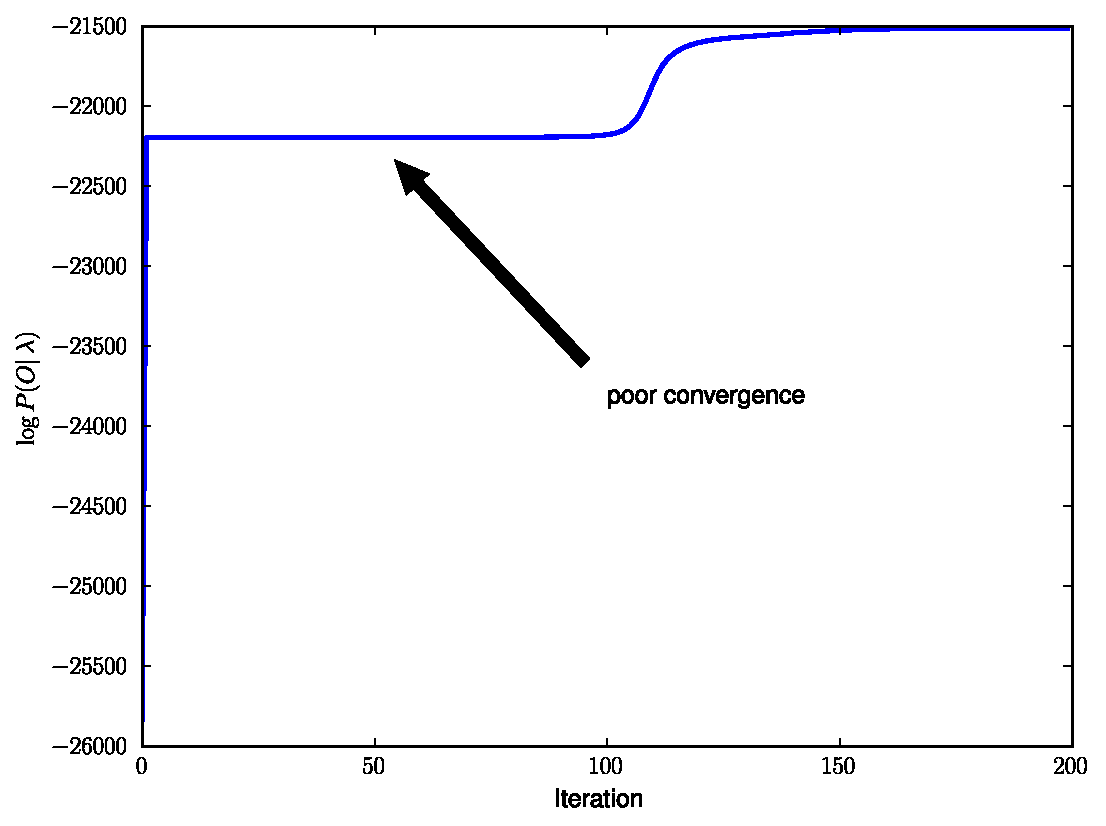
\includegraphics[width=\textwidth]{logProbs.pdf}
\caption{The log probabilities for a HMM trained on the Declaration of Independence
data with 200 iterations. It takes over 100 iterations for the algorithm to work itself out
of a poor local maximum.}
\label{fig:logprobs}
\end{figure}


The learning algorithm is essentially an optimization over the parameter space (i.e. the space of tuples of
stochastic arrays having the proper dimensions) with respect to the objective function $\mathbb{P}(O |\, \lambda)$.
The algorithm is guaranteed to increase the objective function at each iteration, so it is sure to converge.
However, the objective function is riddled with local maxima, and so the outcome depends heavily on the randomly
selected starting values for $A$, $B$, and $\pi$. Figure \ref{fig:logprobs} illustrates the issues involved.
The log probability stays approximately constant for the first 100
iterations. This indicates that the algorithm is not exploring the parameter space enough, and the parameters
found at the 100-th iteration are virtually the same as those found at the first or second iteration. After the first
100 iterations, however, the algorithm is finally able to explore more of the parameter space and hence make
better progress toward increasing the objective function. The moral of the story is that you may need to train
the HMM a few times, using different starting values, and then keep the model that has the highest log likelihood.


\begin{problem}
Implement the learning algorithm by adding the following method to your class:
\begin{lstlisting}
def fit(self, obs, A, B, pi, max_iter=100, tol=1e-3):
    """
    Fit the model parameters to a given observation sequence.

    Parameters
    ----------
    obs : ndarray of shape (T,)
        Observation sequence on which to train the model.
    A : stochastic ndarray of shape (N,N)
        Initialization of state transition matrix
    B : stochastic ndarray of shape (M,N)
        Initialization of state observation matrix
    pi : stochastic ndarray of shape (N,)
        Initialization of initial state distribution
    max_iter : integer
        The maximum number of iterations to take
    tol : float
        The convergence threshold for change in log-probability
    """
    # initialize self.A, self.B, self.pi
    # run the iteration
    pass
\end{lstlisting}
\end{problem}

We now turn to the data found in the file {\tt declaration.txt}.
This file contains the text of the Declaration of Independence.
We will use the sequence of characters (after stripping out punctuation and converting everything to lower-case) as our observation sequence.
In order to convert the raw text into a useable data structure, we need to read in the file, process the string as necessary, and then map the characters to integer values.
We provide sample code below to accomplish this task:
\begin{lstlisting}
>>> import numpy as np
>>> import string

>>> with open("declaration.txt", 'r') as f: # read in the text
>>>     dec = f.read(-1).lower() # convert to lower-case

>>> # next, remove punctuation and newline characters
>>> dec = dec.translate(string.maketrans("",""), string.punctuation+"\n\r")

>>> # create a list of the unique characters in the text
>>> char_map = list(set(dec))

>>> # map each character to its index in char_map
>>> obs = []
>>> for char in dec:
>>>     obs.append(char_map.index(char))
>>> obs = np.array(obs)
\end{lstlisting}

\begin{problem}
You are now ready to train a HMM using the Declaration of Independence data.
Use $N=2$ states and $M=27$ observation values (26 lower case characters and 1 whitespace character),
and run for 200 iterations with the default value for \li{tol}.
Generally speaking, if you converge to a log probability greater than $-21550$, then you have reached
an acceptable set of parameters for this dataset.

Once the learning algorithm converges, analyze the state observation matrix $B$.
Note which rows correspond to the largest and smallest probability values in each column of $B$,
and check the corresponding characters.
The code below displays typical results for a well-converged HMM:
\begin{lstlisting}
>>> for i in xrange(len(h.B)):
>>>     print  "{0}, {1:0.4f}, {2:0.4f}".format(char_map[i], h.B[i,0], h.B[i,1])
 , 0.0051, 0.3324
a, 0.0000, 0.1247
c, 0.0460, 0.0000
b, 0.0237, 0.0000
e, 0.0000, 0.2245
d, 0.0630, 0.0000
g, 0.0325, 0.0000
f, 0.0450, 0.0000
i, 0.0000, 0.1174
h, 0.0806, 0.0070
k, 0.0031, 0.0005
j, 0.0040, 0.0000
m, 0.0360, 0.0000
l, 0.0569, 0.0001
o, 0.0009, 0.1331
n, 0.1207, 0.0000
q, 0.0015, 0.0000
p, 0.0345, 0.0000
s, 0.1195, 0.0000
r, 0.1062, 0.0000
u, 0.0000, 0.0546
t, 0.1600, 0.0000
w, 0.0242, 0.0000
v, 0.0185, 0.0000
y, 0.0147, 0.0058
x, 0.0022, 0.0000
z, 0.0010, 0.0000
\end{lstlisting}
What do you notice about the second column of $B$? It seems that the HMM has detected a vowel state and a consonant state, without any prior input from an English speaker.
Interestingly, the whitespace character is grouped together with the vowels. A HMM can also detect the vowel/consonant distinction in other languages. It appears that
this distinction is a statistically significant aspect of much of human language.
\end{problem}




